\documentclass[main.tex]{subfiles}
\begin{document}
\section{Projektplanung}

Der erste Schritt für die Realisierung des Projektes lag im Verstehen des CTU13-Datensatzes und seinen Besonderheiten (siehe Kapitel 3 Der Datensatz CTU13). Nachfolgend wurden die Machine Learning Algorithmen, die für das Intrusion Detection System in Frage kommen könnten, recherchiert und unter Berücksichtigung der Besonderheiten des CTU13-Datensatzes wurde schließlich ein Algorithmus ausgewählt. Nach dieser Vorarbeit wurde mit der Aufbereitung des CTU13-Datensatzes und anschließend mit der Implementierung des Intrusion Detection Systems begonnen (siehe Kapitel 4 Aufbau des Intrusion Detection Systems). Neben den kontinuierlichen Verbesserungen des IDS war die Evaluierung des IDS die Hauptaufgabe nach der Implementierung des IDS(siehe Kapitel 6 Evaluierung des IDS). 
Die einzelnen Arbeitspakete und ihre Interdependenzen sind in dem nachfolgenden Ablaufdiagramm abgebildet. 
%Ablaufdiagramm 

\begin{figure}[ht]
 \centering
 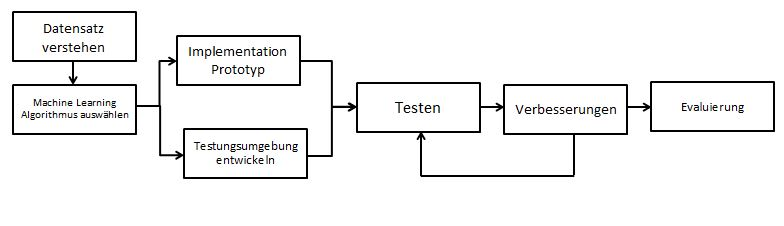
\includegraphics[width=1\textwidth]{images/Ablaufdiagramm.JPG}
 \caption{Ablaufdiagramm}
 \label{Ablaufdiagramm}
\end{figure}


\end{document}


